\documentclass[class=report,crop=false, 12pt]{standalone}
\usepackage[screen,nosolutions]{../myscratch}
%\usepackage[screen]{../myscratch}


\begin{document}

\titre[S]{Si ... alors ...}
%===============================

\insertvideo{pHK3fOJ52Ls}{Si ... alors ... -- Activité 1}

\insertvideo{zXS6NXVUeiQ}{Si ... alors ... -- Activité 2}

\insertvideo{m0YvDz-f3SE}{S i... alors ... -- Activité 3}

\bigskip
\bigskip

\begin{activite}

Scratch se déplace et rebondit sur les bords, il doit atteindre la zone ovale rouge sans toucher les rectangles bleus. Pour cela, il faut choisir la bonne orientation initiale.

\begin{center}
  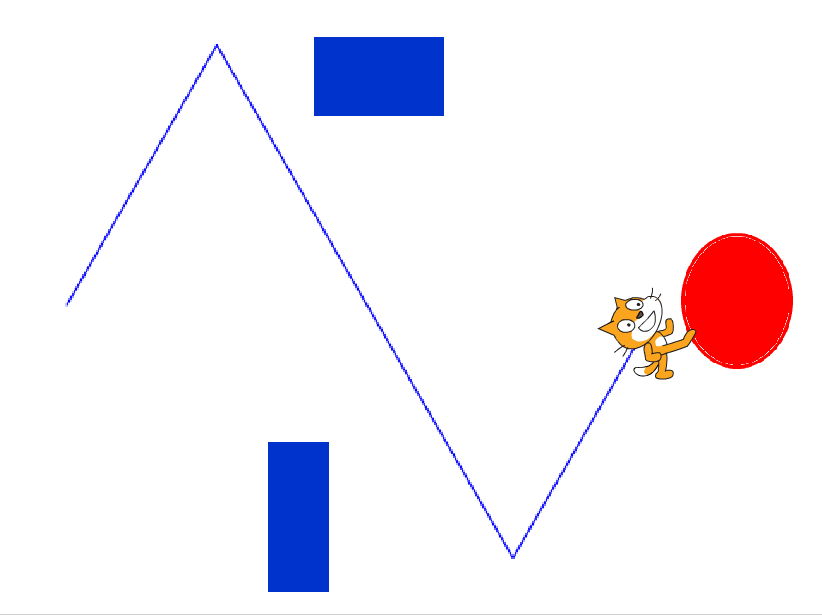
\includegraphics[width=0.6\textwidth]{ecran-04-ex1} 
\end{center}

\begin{enumerate}
  \item Scratch part de $x=-200$, $y=0$. Il s'oriente selon un certain angle (par exemple $30$\textdegree). Puis dans une boucle sans fin \og répéter indéfiniment \fg{}, il avance un peu (disons $5$ pas) et il \og rebondit si le bord est atteint \fg{}.
  
  
  \item Complète la boucle précédente pour tester si Scratch touche une zone colorée :
  \begin{itemize}
    \item si Scratch touche une zone ovale rouge alors c'est gagné et on arrête le programme,
    
    \item si Scratch touche une zone rectangulaire bleue alors c'est perdu et on arrête aussi le programme.
  \end{itemize}
   
  \item Dessine des obstacles (en bleu) et une cible (en rouge) sur l'arrière-plan. Cherche l'angle de départ qui convient à la fois pour éviter les obstacles et pour atteindre la cible !
\end{enumerate}



\textbf{Blocs utiles.}
\begin{center}
\begin{scratch}
  \blockif{si \boolsensing{couleur \pencolor{blue!75!black} touchée ?} alors }
  { 
    \blockspace
  }
\end{scratch}
\qquad\qquad\qquad
\begin{scratch}
  \blockmove{rebondir si le bord est atteint}
  \blockspace
  \blockcontrol{stop \selectmenu{tout}}
\end{scratch}
\end{center}
Afin de choisir exactement les mêmes couleurs que celles utilisées pour dessiner les obstacles ou la cible, utilise la pipette.

\end{activite}



\begin{activite}

L'utilisateur déplace Scratch avec les touches de flèches du clavier de façon à suivre un chemin.

\begin{center}
  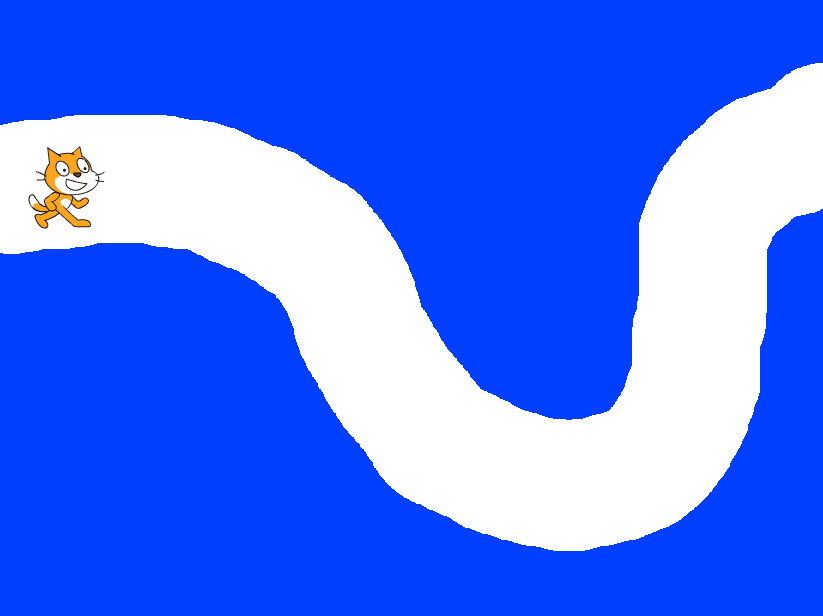
\includegraphics[width=0.47\textwidth]{ecran-04-ex2} 
\end{center}

\begin{enumerate}
  \item Dans une boucle sans fin, on teste quelle flèche est pressée.
  Si c'est la flèche du haut, Scratch monte (de 5 pas par exemple). Si c'est la flèche du bas, Scratch descend...
  
  \item Dessine un parcours sur l'arrière-plan : tout d'abord dessine un grand rectangle tout bleu qui recouvre tout ; puis avec l'outil gomme (en grande taille) trace un chemin.
  
  \item Réduis la taille du lutin Scratch afin qu'il puisse parcourir le chemin sans toucher les bords colorés.
  
  \item \textbf{Bonus.} Si Scratch sort de son chemin, joue un son d'alerte.
\end{enumerate}


\textbf{Blocs utiles.}
\begin{center}
\begin{scratch}
  \blockif{si \boolsensing{touche \selectmenu{ flèche droite} pressée ?} alors }
  { 
    \blockspace
  }
\end{scratch}
\end{center}


\end{activite}

\begin{activite}

Il s'agit de programmer un jeu : 
\begin{itemize}
  \item Scratch part de la gauche de l'écran, il est visible.
  \item Au bout de quelques pas, il disparaît mais continue d'avancer. 
  \item Lorsque le joueur appuie sur le bouton gauche de la souris, Scratch s'arrête et réapparaît.
  \item Si Scratch touche la barre noire à ce moment là, c'est gagné !
\end{itemize}

\begin{center}
  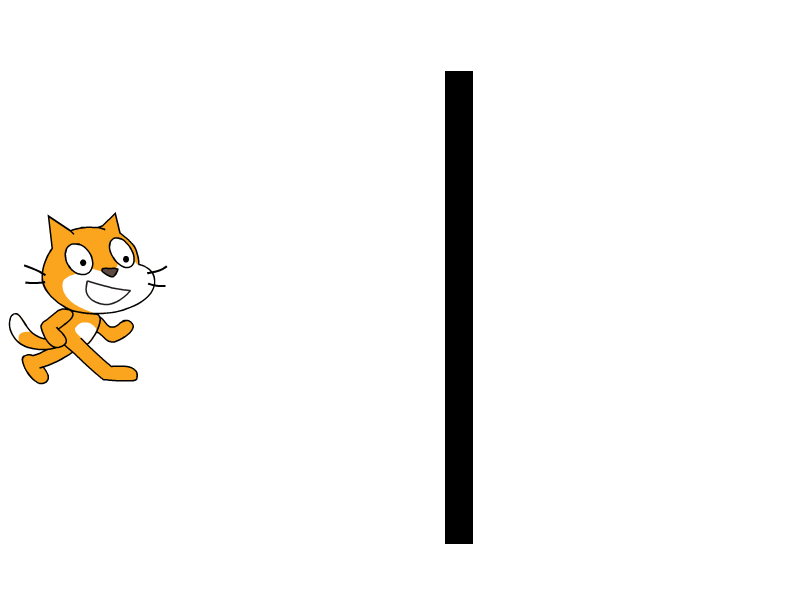
\includegraphics[width=0.42\textwidth]{ecran-04-ex3} 
\end{center}

Dans un premier temps, modifie l'arrière-plan pour y dessiner une barre verticale noire vers le milieu de l'écran.

\begin{enumerate}
  \item \textbf{Première partie.} Scratch démarre.
  
  \begin{itemize}
    \item Positionne Scratch à gauche de l'écran, visible.
    \item Répète 10 fois : Scratch avance de 5 et attend un peu (par exemple 0,1 seconde). 
  \end{itemize}
  
  
  \item \textbf{Deuxième partie.} Scratch se cache.
  
  \begin{itemize}
    \item Cache Scratch.
    \item Répète 70 fois : Scratch avance de 5 et attend un peu (le même temps qu'avant). 
  \end{itemize}
  
  \item \textbf{Troisième partie.} Le joueur clique.
  
  À chaque itération de la boucle précédente, on teste si le bouton gauche de la souris est pressé. Si le joueur clique sur la souris alors :
  \begin{itemize}
    \item montre Scratch,
    \item si Scratch touche la barre noire alors affiche : \og c'est gagné ! \fg{},
    \item arrête le programme.
  \end{itemize}  

\item \textbf{Quatrième partie.} Le joueur ne clique pas.

  Si le joueur n'a pas cliqué lors de la boucle alors Scratch se montre et dit \og{}Trop tard !\fg{}.
  
\end{enumerate}

\bigskip
\textbf{Blocs utiles.}
\begin{center}
\begin{scratch}
  \blockif{si \boolsensing{souris pressée ?} alors }
  { 
    \blockspace
  }
\end{scratch}
\qquad
\begin{scratch}
  \blockif{si \booloperator{couleur \pencolor{blue!75!black} touchée ?} alors }
  { 
    \blockspace
  }
\end{scratch}
\qquad
\begin{scratch} 
  \blocklook{montrer}
  \blockspace[0.7]
  \blocklook{cacher}
  \blockspace[0.7]
  \blockcontrol{stop \selectmenu{tout}}
\end{scratch}
\end{center}

\end{activite}



\ifx \displaysolutions \myzero
\else
\begin{code}
\setscratch{scale=0.45}
\onesolution{Si ... alors ...}{Activité 1}{
\begin{scratch}
  \blockinit{quand \greenflag est cliqué}
  \blockmove{aller à x: \ovalnum{-200} y: \ovalnum{0}}
  \blockmove{s'orienter à \ovalnum{30}}
  \blockinfloop{répéter indéfiniment}
  {
    \blockmove{avancer de \ovalnum{5} pas} 
    \blockmove{rebondir si le bord est atteint}
    \blockif{si \boolsensing{couleur \pencolor{red!75!black} touchée ?} alors }
    { 
      \blocklook{dire \ovalnum{ Gagné !} pendant \ovalnum{2} secondes}
      \blockcontrol{stop \selectmenu{tout}}
    }
    \blockif{si \boolsensing{couleur \pencolor{blue!75!black} touchée ?} alors }
    { 
      \blocklook{dire \ovalnum{ Perdu !} pendant \ovalnum{2} secondes}
      \blockcontrol{stop \selectmenu{tout}}
    }    
   }
\end{scratch}
}
\onesolution{Si ... alors ...}{Activité 2}{
\begin{scratch}
  \blockinit{quand \greenflag est cliqué}
  \blockmove{aller à x: \ovalnum{-200} y: \ovalnum{80}}
  \blockmove{s'orienter à \ovalnum{90}}
  \blockinfloop{répéter indéfiniment}
  {
    \blockif{si \boolsensing{touche \selectmenu{ flèche droite} pressée ?} alors }
    { 
      \blockmove{ajouter \ovalnum{5} à x}
    }
    \blockif{si \boolsensing{touche \selectmenu{ flèche gauche} pressée ?} alors }
    { 
      \blockmove{ajouter \ovalnum{-5} à x}
    }
    \blockif{si \boolsensing{touche \selectmenu{ flèche haut} pressée ?} alors }
    { 
      \blockmove{ajouter \ovalnum{5} à y}
    }
    \blockif{si \boolsensing{touche \selectmenu{ flèche bas} pressée ?} alors }
    { 
      \blockmove{ajouter \ovalnum{-5} à y}
    }    
   }
\end{scratch}
}
\onesolution{Si ... alors ...}{Activité 3}{
\begin{scratch}
  \blockinit{quand \greenflag est cliqué}
  \blockmove{aller à x: \ovalnum{-240} y: \ovalnum{0}}
  \blockmove{s'orienter à \ovalnum{90}}
  \blocklook{montrer}
  \blockrepeat{répéter \ovalnum{10} fois}
  {
    \blockmove{ajouter \ovalnum{5} à x}
    \blockcontrol{attendre \ovalnum{0.1} secondes} 
  }
  \blocklook{cacher}
  \blockrepeat{répéter \ovalnum{70} fois}
  {
    \blockmove{ajouter \ovalnum{5} à x}
    \blockcontrol{attendre \ovalnum{0.1} secondes}
    \blockif{si \boolsensing{souris pressée ?} alors }
    { 
      \blocklook{montrer}
      \blockif{si \boolsensing{couleur \pencolor{black} touchée ?} alors }
      {
      \blocklook{dire \ovalnum{ Bravo !} pendant \ovalnum{2} secondes}
      }
      \blockcontrol{stop \selectmenu{tout}}
    } 
  }
  \blocklook{montrer}
  \blocklook{dire \ovalnum{ Trop tard !}}
\end{scratch}
}    
\end{code}
\fi



\end{document}

